\documentclass{article}

% Lenguaje y Fuente
\usepackage[spanish]{babel}
\usepackage[utf8x]{inputenc}
\usepackage[T1]{fontenc}
\usepackage[top=1in, bottom=1.25in, left=1.1 in, right=1.1 in]{geometry}
\usepackage{graphicx}
\usepackage{ragged2e}
\usepackage[usenames]{color}
\usepackage{multicol}

% Portada

\title{\textbf{Evaluación 2}\\ Cálculo de la Evapotranspiración de Referencia $ET_0$}
\author{Luis Fernando Duarte Gonzalí \\ Universidad de Sonora \\ Física Computacional}
\date{5 de Mayo del 2019}
\begin{document}
\maketitle

% Contenido del Reporte

\section{Introducción}
En la agricultura existe un área encargada de la planeación de irrigación de cultivos o uso de agua, en el cual se estudia la cantidad de vapor de agua en la atmósfera, que no proviene sólo de la evaporación del agua de océanos, ríos o lagos, también de la procedente de la humedad del propio suelo, así como también la transpiración de las plantas. A todo este proceso se le llama Evapotranspiración.

\subsection{Evapotranspiración}

La Evapotranspiración de referencia $ET_0$, es uno de los parámetros mas importantes en los estudios hidrológicos, ambientales y agrícolas y juega un papel muy importante en los proyectos de manejo de irrigación y uso de agua en la agricultura. La ET0 es estimada por diversos métodos: utilizando lisímetros, sistemas de covariancias turbulentas o utilizando métodos indirectos utilizando variables climáticas. 

El requerimiento de conocer un conjunto de valores de las variables climáticas ha sido una de las limitantes de la aplicación de la Ecuación de Penman-Monteith. Por ello se han desarrollado toda una serie de ecuaciones para el cálculo alternativo de la ET0 bajo diversas condiciones climáticas. En esta actividad nos daremos la tarea de evaluar cuáles son las mejores alternativas de la ecuación de Penman-Monteith para una región climática como la nuestra (zona semiárida seca).

\section{Parte 1}
En esta actividad vamos a trabajar con datos meteorológicos del viñedo que se encuentra ubicado en el kilómetro 41 de la carretera de Hermosillo a Bahía Kino (Latitud 28º 55.117' N, Longitud 111º 18.638' W, altitud 101m.

Después de haber leído o por lo menos visto un poco del artículo de Djaman y el reporte 56 de la FAO, trataremos de aplicar los principales resultados de ese estudio y haremos un contrate con los datos que tenemos del viñedo ubicado cerca de Hermosillo.

Con los datos meteorológicos que se tienen, se construyó una tabla de promedios mensuales similar a la Tabla 1 de Djaman:
\begin{center}
    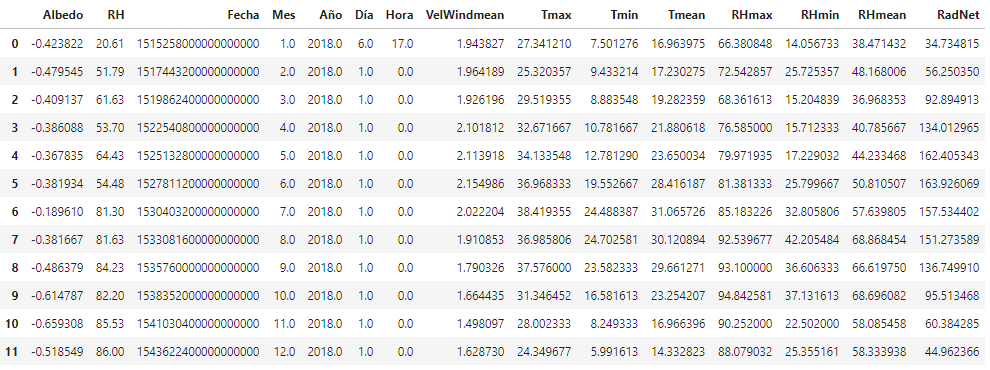
\includegraphics[width = \textwidth]{Tabla.png}
\end{center}
Donde el mes de enero está representado por el número 0 en la columna de índices, a la cual le corresponden todos los datos de esa fila y así sucesivamente.

En esta misma parte, con la información de la tabla se generaron 3 gráficas con matplotlib.

\subsubsection*{Evolución de las Temperaturas}
\begin{center}
    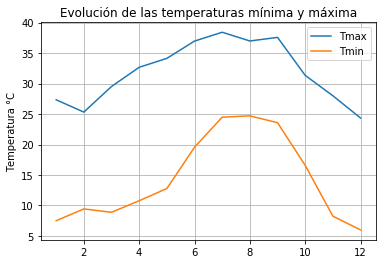
\includegraphics[scale = 0.58]{Temp.png}
\end{center}
Donde se puede observar que los meses más calurosos van desde el mes de Junio a Septiembre que es el periodo de verano. Y también se ve que los meses más fríos son los que se encuentran en el periodo de invierno.

\subsubsection*{Humedad Relativa}
\begin{center}
    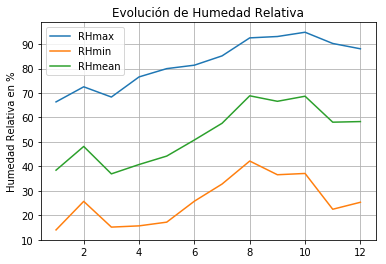
\includegraphics[scale = 0.58]{RH.png}
\end{center}
En esta gráfica se observa mayor humedad relativa en los meses que pertenecen al periodo de primavera y verano donde el calor es mayor y por lo tanto hay más evaporación del agua.

\subsubsection*{Radiación Solar}
\begin{center}
    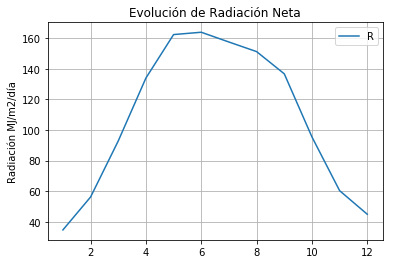
\includegraphics[scale = 0.6]{Rad.png}
\end{center}
Donde se observa mucha menor radiación en los meses pertenecientes al periodo de invierno (Diciembre-Marzo).

\section{Parte 2}
En esta parte seguimos trabajando con los datos anteriores, pero ahora para calcular la Evapotranspiración $ET_0$ mensual promedio utilizando las ecuaciones de los siguientes 3 autores que aparecen en el artículo de K. Djaman:
\\

\textbf{Ecuación 7, Jansen \& Haise (1963)}
\begin{equation}
    ET_0 = (0.0252 T + 0.078) Rs
\end{equation}

\textbf{Ecuación 31, Valiantzas 1 (2012)}
\begin{equation}
    ET_0 = 0.0393 Rs (T_{mean} + 9.5)^{0.5} - 0.19 Rs ^{0.6} \phi ^{0.15} + 0.0061 (T_{mean} + 20)(1.12 T_{mean} - T_{min}-2)^{0.7}
\end{equation}
Donde $\phi$ es la latitud en radianes.
\\

\textbf{Ecuación 34, Valiantzas 4 (2013)}
\begin{equation}
    ET_0 = 0.051 (1 - \alpha) Rs (T_{mean} + 9.5)^{0.5}-2.4\bigg(\frac{Rs}{Ra}\bigg)^{2} + 0.048 (T_{mean} + 20)\bigg(1-\frac{RH}{100}\bigg)(0.5+0.536 u 2) + 0.00012z
\end{equation}
donde $\alpha$ es el albedo, $Ra$ es la radiación solar en la parte alta de la atmósfera $u2$ es la velocidad del viento a 2 m de altura, $z$ es la altura sobre el nivel mar.
\clearpage

La tabla obtenida con los datos de promedios mensuales fue la siguiente:
\begin{center}
    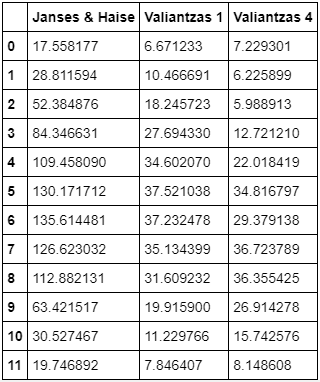
\includegraphics[scale = 0.7]{Tabla2.png}
\end{center}

\section{Parte 3}
En esta parte usamos el archivo de "FlujosVid18.csv". A través de un Balance de Energía también es posible determinar la fracción de Evapotranspiración o Calor Latente $\lambda ET$ mediante la ecuación:

\begin{equation}
    Rn - G - \lambda ET  - H  = 0
\end{equation}
Donde $Rn-G$ es la radiación neta ($Rg_f$), $\lambda ET$  es el calor latente ($LE_f$) y H es el calor sensible ($H_f$).

Con los datos leídos, se produjo una gráfica del balance energía promedio en un mes típico (promedio por hora en un mes).

\begin{center}
    \includegraphics[scale = 0.6]{Energia.png}
\end{center}

\section{Referencias}

\begin{itemize}
    \item Evaluation of the Penman-Monteith and other 34 reference evapotranspiration equations under limited data in a semiarid dry climate (2018). Consultado el 5 de Mayo del 2019, de Theoretical and Applied Climatology. Sitio web: 
    
    https://link.springer.com/article/10.1007\%2Fs00704-018-2624-0
\end{itemize}




\end{document}
